In order to find $A_{i1}$ and $A_{i2}$, we started to implement the disturbance to the SIMULINK model (see figure \ref{fig:linearModelNoise}).

\begin{figure}[H]
 \centering 
 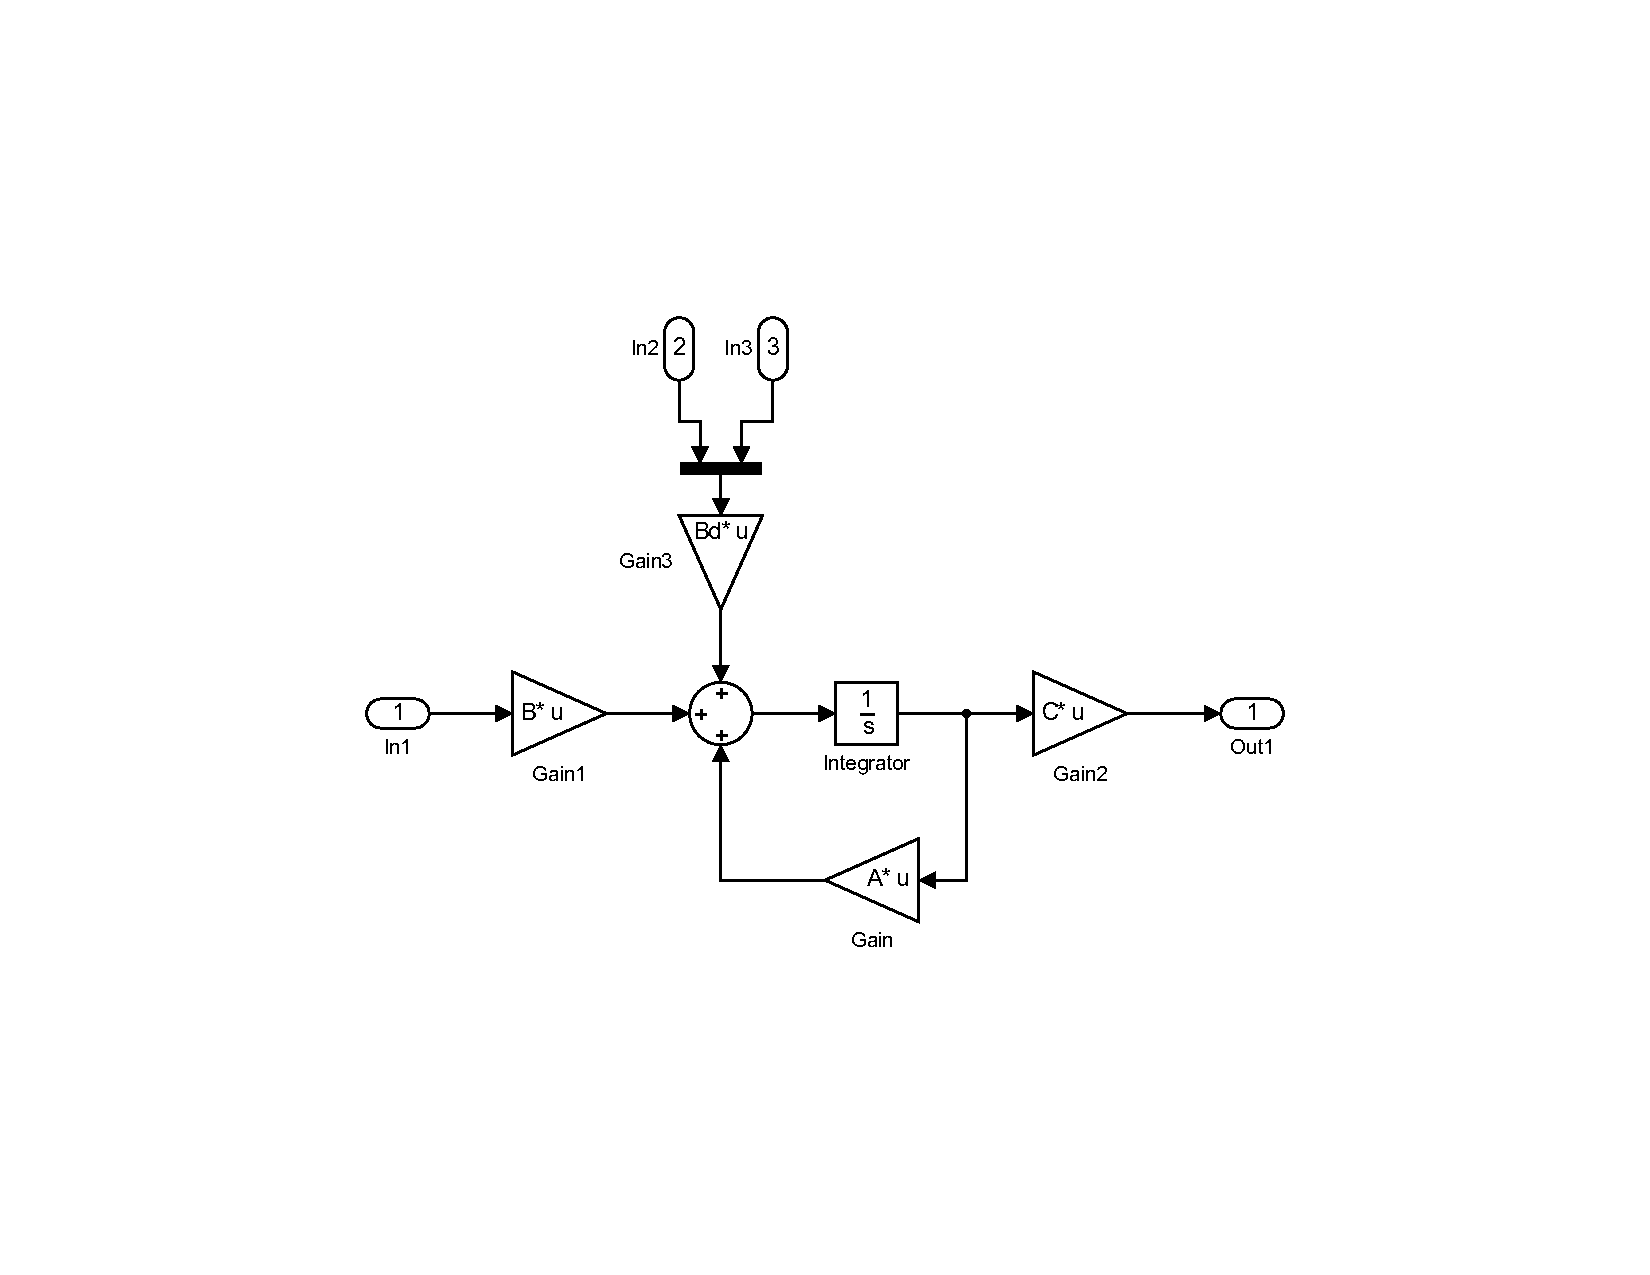
\includegraphics[trim=5cm 5cm 2cm 5cm, clip=true, totalheight=0.35\textheight, angle=0]{figures/linearModelNoise.pdf}
 \caption{SIMULINK model of the linearised loudspeaker with noise}
\label{fig:linearModelNoise}
\end{figure}

Then, we have chosen $A_{i1}=5V$ and run the simulation to see the magnitude of the speak at 40$Hz$: $magnitude_{40Hz} = 0.2288\ V$. Knowing that the magnitude wanted is 0.0038 $V$ (determined with the nonlinear Model), we can find $A_{i1}=\frac{5*0.0038}{0.2288}=0.0830\ V$. In the same way, we find $A_{i2}=?\ V$.